% !TeX root = ../thuthesis-example.tex

\chapter{具备策略库的网络任务规划范式设计}
\section{本章序言}
在网络领域,有许多重要的任务,包括拥塞控制、可变比特率控制和梯度压缩任务,这些任务在过去几十年中积累了众多有效的方法。例如,在拥塞控制任务中,有基于简单规则的算法(如 Cubic \cite{ha2008cubic},基于丢包的算法,以及 BBR \cite{cardwell2016bbr},基于带宽-延迟积的算法),也有基于人工智能的方法,如强化学习(例如 Sage\cite{yen2023computers})或在线学习(例如 PCC Vivace\cite{dong2018pcc})。这些任务涉及许多策略,形成了各自的“策略库”,这些策略库是经过数十年努力和不断完善的结果,由无数学者创造,最终形成了一套可以应用于各种场景的强大算法集合。大多数方法基于不同的设计原则,具有不同的性能和适用性,能够适应不同的网络环境和需求。部分算法的统计如表\ref{table_task_algo}所示。

然而,在传统的网络传输控制范式中,大多数连接在建立时采用固定的控制策略。以拥塞控制为例:在绝大多数Linux个人主机上,默认使用Cubic算法,除非用户手动切换算法。即便在数据中心,通常也会配置固定策略以确保服务的稳定性,所有连接都会使用单一的控制方法。这个经典范式的缺点在于依赖于单一策略,即使网络特性可能更适合采用不同的策略,从而缺乏多样性。事实上,由于每种拥塞控制算法设计原则的不同,不论一个策略多么强大,它都会因为设计上的局限性而表现出局部性和偏差,无法涵盖所有网络条件,在某些场景下可能会陷入局部最优解。

为了避免陷入这种困境,最直观的方法是根据网络状况手动为每种情况选择一个策略。然而,这种做法的成本远大于其收益。在过去几十年里,一些研究致力于转变这种传统范式。例如,Remy \cite{winstein2013tcp} 通过利用关于网络的先验知识或假设,旨在生成一种拥塞控制策略。Sage \cite{yen2023computers} 试图通过离线强化学习来学习各种算法的“优势”,从而在大多数场景中表现出优于其他算法的效果。另一方面,Antelope \cite{zhou2022machine} 提出了一个避免设计“千篇一律”算法的系统,而是根据情况在“最适合”的控制算法之间切换。尽管这些范式具有开创性,但它们仍然受到个别算法性能的局限性或从多种算法中选择的瓶颈所制约。

然而,近年来,大型语言模型(Large Language Models,LLMs)的出现为转变这一旧有范式提供了新的机遇。许多研究证明,LLMs在环境感知理解、规划和决策方面具备强大的能力,这一点通过LLMs代理的崛起得到了体现,并且它们已经在工具规划中得到了应用。此外,通过适当的微调和设计技术,这些LLMs还可以在特定领域进一步提升其性能。LLMs所展现出的决策能力也表明,它们有潜力感知网络环境、理解应用需求,并做出相应的规划。

受到此启发,本工作提出了一种新的范式,在这种范式中,对于任何类型的网络决策任务,预训练的LLMs 根据网络状况从策略库中选择“最适合”的策略,从而实现动态的宏观层级策略切换,增强算法选择的适应性。

构建这一范式面临以下挑战:

\begin{itemize} \item \textbf{改变范式及LLM对网络状况的感知。}目前的网络控制算法和协议缺乏在连接建立过程中切换方法的能力,因此需要重新定义工作流程,增加一个切换控制策略的步骤。此外,网络系统需要增强感知趋势、通用信息和应用层需求的能力。

\item \textbf{网络策略决策的独特性。}常见的规划任务通常在静态环境中运行,任务可以通过链式思维(Chain-of-Thought)等技术进行分解,并通过即时反馈(如人工反馈或环境反馈)加以解决。然而,在网络任务中,决策难以明确分解,且反馈在决策之后延迟出现。此外,环境是非确定性的,存在概率性变化。因此,LLM在网络场景中的规划能力与传统的LLM规划方法有所不同。

\item \textbf{LLM获取网络决策经验的问题。}尽管预训练的LLM拥有丰富的知识,但它们仍然缺乏在网络策略选择和决策中做出有效选择的能力。目前所获得的知识尚不足以使LLM在这一背景下始终做出有价值的决策。 
\end{itemize}

针对上述挑战,本工作的主要设计思路包括一个新的范式,该范式结合了使用特定技术微调的LLM和修改后的系统工作流程。

为了使模型具备选择策略的能力,该工作将策略规划问题视为强化学习任务,并利用决策变换器(Decision Transformer)的离线强化学习框架 \cite{chen2021decision},为模型学习提供机制。该工作使用LoRA方法来训练模型中部分变量权重,并通过模型微调(Supervised Fine-Tuning,SFT)来提升规划性能。

为了感知网络趋势的变化,该工作设计了一个针对多维网络时间序列数据的自定义嵌入层,使工作能够提取任务在较长时间段内的时序语义。

此外,该工作引入了网络系统与策略规划系统之间的交互机制,使得不同的策略和算法可以在执行过程中灵活切换,以更好地适应当前状态。


\section{网络领域策略性控制的范式背景}
在网络领域,许多任务需要策略性控制,以提高网络利用率并确保质量保障。自适应码率流媒体(Adaptive Bitrate Streaming,ABR)、拥塞控制(Congestion Control,CC)和梯度压缩(Gradient Compression,GC)等任务占据了大部分网络流量,并且是关键的质量保障节点。因此,过去几十年里,针对这些领域进行了大量研究,不断引入新的方法和思想。这些研究和工程实现最终形成了一个庞大的算法库,这些算法在不同的原理和工作机制下运行。一些经典算法列在表\ref{table_task_algo} 中。

\begin{table}[htbp]
\centering
\caption{网络环境中的重要任务关键性能指标及经典控制策略}
\resizebox{\columnwidth}{!}{%
\begin{tabular}{@{}ccccc@{}}
\toprule
\textbf{任务}                                          & \textbf{关键性能指标}                                & \textbf{策略} & \textbf{原理} & \textbf{年份} \\ \midrule
\multirow{6}{*}{\textbf{自适应码率流媒体}} & \multirow{6}{*}{重缓冲、码率、平滑性} & Pensieve \cite{mao2017neural}          & 基于强化学习            & 2017          \\
                                                       &                                              & Genet \cite{xia2022genet}            & 基于强化学习            & 2022          \\
                                                       &                                              & MPC               & 动态规划                  & 2015          \\
                                                       &                                              & BBA               & 基于缓冲区        & 2014          \\
                                                       &                                              & BOLA \cite{spiteri2020bola}             & 基于缓冲区        & 2016          \\
                                                       &                                              & NetLLM \cite{wu2024netllm}            & 基于Transformer   & 2024          \\ \midrule
\multirow{6}{*}{\textbf{拥塞控制}}           & \multirow{6}{*}{吞吐量、丢包、延迟}    & CUBIC \cite{ha2008cubic}             & 基于丢包          & 1990年代         \\
                                                       &                                              & Reno              & 基于丢包          & 1990年代         \\
                                                       &                                              & WestWood \cite{casetti2002tcp}          & 基于丢包          & 2002          \\
                                                       &                                              & BBR \cite{cardwell2016bbr}
                                                    & 带宽延迟积                 & 2015          \\
                                                       &                                              & Aurora \cite{jay2019deep}            & 基于强化学习            & 2019          \\
                                                       &                                              & Sage \cite{yen2023computers}             & 基于强化学习            & 2023          \\ \midrule

\multirow{2}{*}{\textbf{梯度压缩}}         & \multirow{2}{*}{压缩率、准确度、效率}                            & Top-K             & 稀疏化           & 2010年代        \\
                                                    
                                                       &                                              & DC2 \cite{abdelmoniem2021dc2}             & 基于延迟    &   2021            \\ \bottomrule
\end{tabular}
}
\label{table_task_algo}
\end{table}


这些任务的介绍如下:

\textbf{自适应码率:} 主要用于视频流媒体,基于实时网络状况自动调整视频质量,以确保流畅播放并优化用户体验,尤其是在带宽波动时。

\textbf{拥塞控制:} 旨在通过动态调整数据传输速率来避免网络过载,从而提高网络稳定性和效率,即使在高流量条件下也能确保良好的服务质量。

\textbf{梯度压缩:} 在模型训练过程中减少传输的梯度信息的大小,以降低通信成本并提高分布式训练的效率,通常用于训练大规模深度学习模型。

然而,由于这些方法的工作原理和设计理念不同,算法在不同网络环境中的表现也各不相同。没有单一的算法能够在所有网络条件和场景中始终表现出优越的性能。以自适应码率流媒体场景作为验证,该工作使用累积奖励值来评估算法在随机网络环境中的表现。累积奖励的计算方式如式\eqref{eq:abr_cum_reward}所示:

\begin{equation}
\begin{aligned}
    \sum_i(\alpha \cdot Rebuf_i + \beta \cdot Bitrate_i + \gamma \cdot BitrateChange_i) \cdot \frac{1}{n}
\end{aligned}
\label{eq:abr_cum_reward}
\end{equation}

较高的累积奖励值表示更好的性能。测试结果如图\ref{fig_manual_switch} 所示。该工作使用genet策略进行测试,如紫色线所示,并观察到当网络遇到波动时,会导致显著的奖励损失,从而导致累积奖励的下降。相比之下,在该工作构建的可切换系统中,使用随机选择功能随机选择的算法能够缓解对整体累积奖励的影响,如橙色线所示。基于预先手动选择和切换算法的策略表现出了最佳的累积奖励,代表了最优性能,如棕色线所示。

\begin{figure} [h!]
\centering
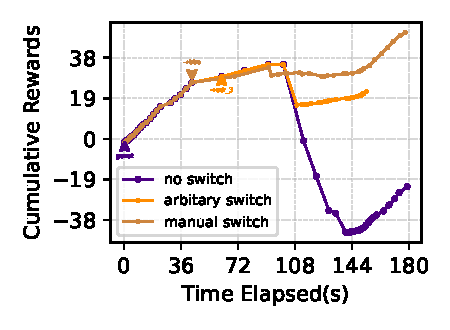
\includegraphics[width=0.5\linewidth]{figures/chap04/manual_switch_validation.pdf} 
\caption{策略切换带来的性能改变}
\label{fig_manual_switch}
\end{figure}



\section{范式更新的设计动机}
绝大多数网络任务在环境变化的情况下,仍然使用单一策略持续运行。这一直是常见的采用模式。在这种背景下,许多强大的算法得到了开发。然而,迄今为止,没有任何单一策略能够在所有网络环境中表现出色,或者在每个场景中展示最优性能,这主要是由于它们设计原理的差异。为特定条件优化的策略已经被创造出来,使得它们能够在这些特定场景中表现优异。然而,尽管通用算法可能适用于更多场景,它们通常不如针对性策略表现得那么好;相反,针对性策略可能不具有如此广泛的适用性。人们必须接受的关键观点是:策略必须在针对性优化和通用性之间找到平衡,而不可能同时实现两者的极致最优。

事实上,这个丰富且适应性强的策略库在过去几十年中通过一系列战略性进展无意间建立起来了。能否开发一种方法,利用这个库中各种策略的优势,同时避免它们的弱点?一种直观的方法是,在合适的时机从这个库中选择最适合的策略,并在必要时进行切换,如图\ref{fig_paradigm_change} 所示。图中最下方的“环境”代表客观环境的波动,在图中网络状况被分成了三段。过去的范式采用一成不变的规则,而新的范式支持在策略库中根据网络环境的变化采取切换的措施。

\begin{figure} [ht]
\centering
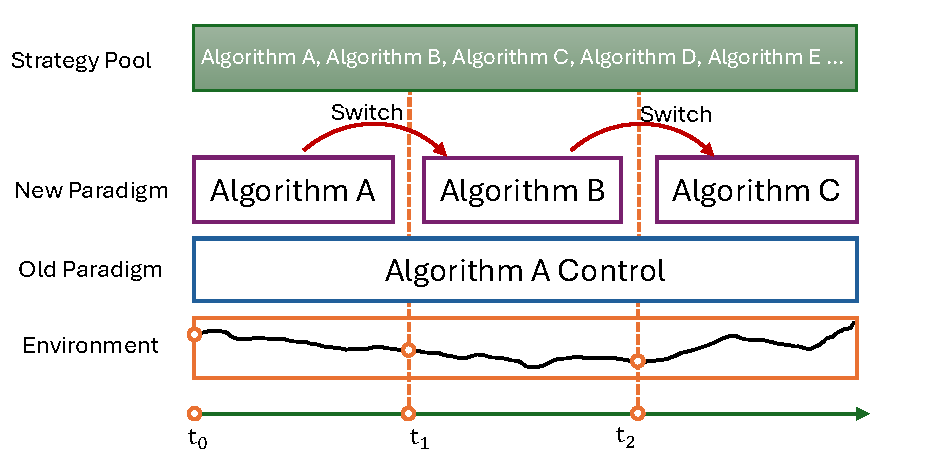
\includegraphics[width=0.7\textwidth]{figures/chap04/Paradigm_change.pdf} 
\caption{新范式利用算法库在网络环境变化时进行策略切换}
\label{fig_paradigm_change}
\end{figure}

然而,实现该工作范式将在构建时会面临下列挑战和问题:

\textbf{如何进行策略规划?} 最简单的实现和验证方法是通过手动或使用简单规则来监控和评估当前环境,然后根据策略的设计原理,从策略库中选择和配置最合适的策略。通过手动和随机切换的案例,已经证明了这种切换可以带来性能提升。这种方法适用于小规模的演示和效果验证,但显然依靠人工无法总结所有适当的切换规则,而且手动维护的成本太高。

近年来,大型语言模型的出现为转变这一旧有范式提供了新的机会。许多研究已证明,LLMs在环境感知理解、规划和决策方面具有强大的能力,正如LLM代理(LLM Agents)\cite{wang2024survey} 的崛起及其在工具规划中的应用所证明的那样。此外,通过适当的微调和设计技术,这些LLMs可以在特定领域进一步提高其性能。LLMs展示的决策能力也表明,它们有潜力感知网络环境、理解应用需求并制定合适的规划。

\textbf{为什么不使用简单的算法?} 使用基于规则的算法(如决策树)来完成策略规划,缺乏动态更新能力和应对所有条件的能力。该工作的设计期望这个范式能够基于网络环境和动态更新的策略库进行有效规划,包括算法选择和参数配置。这不仅仅是一个简单的分类或回归任务,也没有直接可映射的函数。基于规则的策略将面临与前面例子相同的问题,无法更新并识别所有可能的情况。而LLMs更擅长从人类偏好和需求理解的角度进行思考。

\textbf{为什么不让LLMs生成基于规则的策略?} 由于LLMs的幻觉问题,直接生成规划策略会导致严重的不稳定性。在工具规划工作中,LLM-ABR使用了多个验证机制来确保部分有效的答案,但对于需要高稳定性的网络任务来说,这是不可接受的。此外,直接生成基于规则的策略并不能充分利用随着时间积累起来的大量策略库。

\textbf{为什么不直接使用LLM作为策略?} 主要的限制因素是LLMs的推理延迟。LLM的推理延迟是一个显著因素,因为网络任务需要高实时性性能。如表\ref{tab:infer_latn}所示,LLM的生成延迟常常超过可接受的安全范围。在多款高性能GPU上,模型每个代词(Token)的推理速度仍然会慢于拥塞控制、自适应比特率流、梯度压缩的最高要求,尤其是当生成的代词(Token)数量较多时。类似地,直接使用LLM作为策略生成器也存在超出安全阈值的风险。


\begin{table}[ht]
\caption{大型语言模型推理的时间消耗与网络任务所需时效对比}

\resizebox{\columnwidth}{!}{%
\begin{tabular}{@{}ccccc@{}}
\toprule
项目                              & 模型         & 量化方式   & 运行GPU              & 延迟\cite{colab2023}  \\ \midrule
理论                            & Mistral-7B    & 16位        & RTX 4090(1008 GB/s)      & 14.1ms/Token               \\
理论                            & Mistral-7B    & 8位         & RTX 4090                 & \textbf{7ms/Token}         \\
实际                            & ChatGLM3-6B   & 16位        & RTX 4090(2022)           & 16ms/Token                 \\
实际                            & ChatGLM3-6B   & 16位        & V100 32GB (2017)         & 32ms/Token                 \\
实际                            & Qwen-7B       & 16位        & RTX 4090(2022)           & 19ms/Token                 \\
拥塞控制                          & /             & /              & /                        & 1$\sim$3 RTT (10$\sim$50ms) \\
自适应比特率流                   & /             & /              & /                        & 每个块 (1-5s) \\
梯度压缩                          & /             & /              & /                        & 每次迭代 \\
\bottomrule
\end{tabular}
}
\label{tab:infer_latn}
\end{table}


因此,本工作决定构建一个基于大模型的策略规划方法,该方法在一个能够切换策略的范式内运行。该方法能够有效选择和配置策略,并依赖于一个可靠的过程,在必要时动态切换策略。由于运行中的策略已经经过验证并且稳定,系统保持可靠性和鲁棒性。




\section{网络任务规划范式设计}
在确定利用大模型的决策和规划能力对于网络层面的策略做出宏观调控后,本工作致力于解决将其应用过程中的挑战。为此,本工作设计了LLM-NP(Large Language Model for Network Planning),它提供了利用大模型进行网络规划的范式。LLM-NP运行过程可以使用图\ref{fig_llmcc_design}表示。具体而言,LLM-NP的设计由网络与决策系统的策略选择和交互机制、模型规划能力的习得和调优以及模型对网络变化趋势感知和分析三个重点构成。

\begin{figure} [ht]
\centering
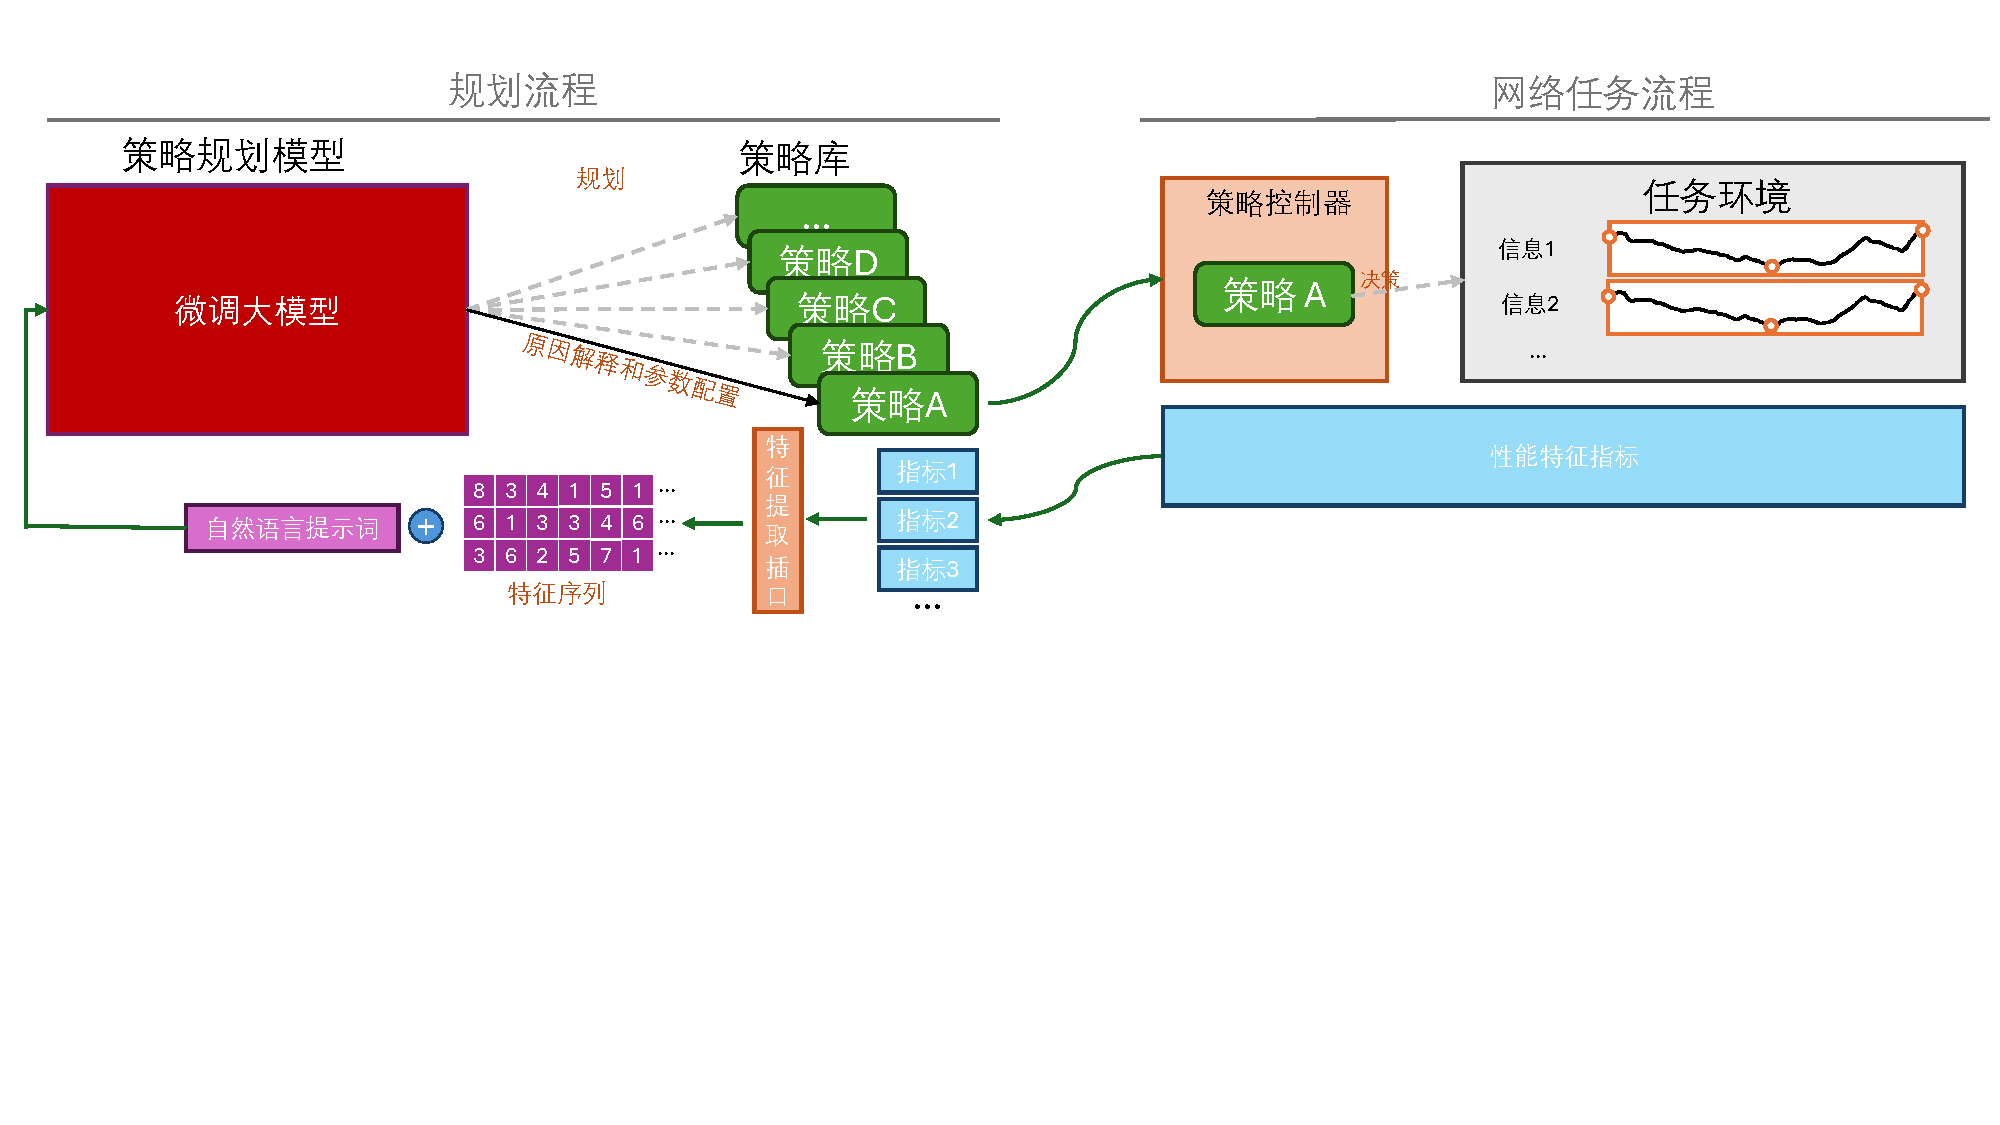
\includegraphics[width=\textwidth]{figures/chap04/design.pdf} 
\caption{网络控制策略选择范式设计概览}
\label{fig_llmcc_design}
\end{figure}


\subsection{网络与决策系统的策略选择和交互机制}
系统运行的整个流程被分为规划流程和网络任务流程。规划流程接收来自于网络任务中的指标反馈,负责在已支持的备选策略库中选择策略,根据当下和先前的网络状态做出合理的规划;而网络任务则可以是任何一个需要进行网络规划的任务。为了适配规划流程,网络任务流程也需要进行调整,以暴露出其从一个算法切换为库中其他算法、和网络状态反馈的接口,如图\ref{fig_llmcc_api}所示。以自适应码率任务为例,流媒体的发送服务器作为一个独立进程工作,并定期将网络状态和工作相关的指标(例如发送的速率、是否遇到缓冲重加载、估计带宽的信息)以网络间进程通信的方式发送给规划进程。规划进程在获得相关指标后使用LLM进行分析,并给出规划的结果,这个结果交由网络任务系统,并在网络任务系统中进行切换。

\begin{figure} [ht]
\centering
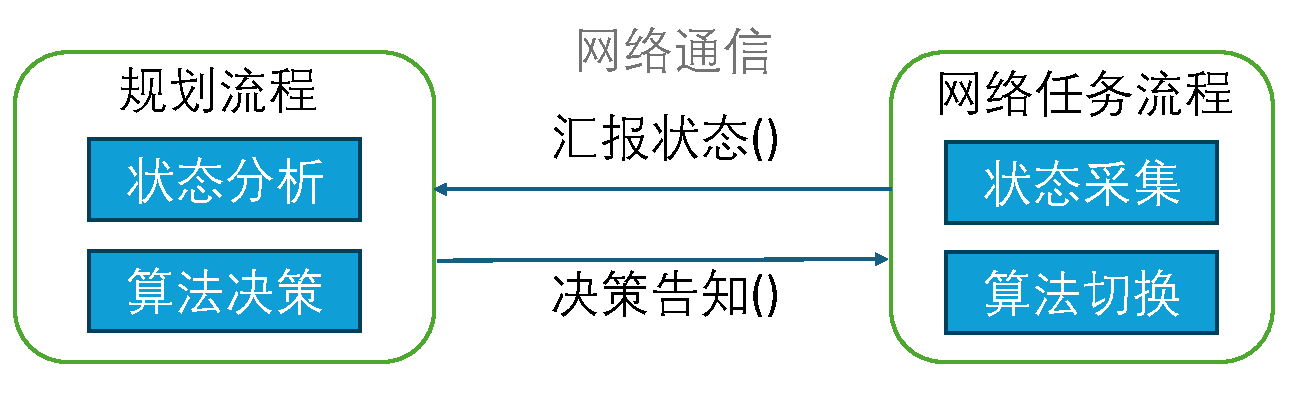
\includegraphics[width=0.65\textwidth]{figures/chap04/API.pdf} 
\caption{规划流程和网络任务流程需开放的接口和交互模式}
\label{fig_llmcc_api}
\end{figure}


这种独立流程的方式有两个好处:

(1)规划进程与网络任务进程独立运行,互不干扰。两者之间通过网络协议通信,可以建立独立的规划服务器运行规划进程,将规划进程独立运作于适合推理硬件性能的服务器上,作为中枢专为网络中心提供合适的架构。对于部份运行环境要求严苛的算法,这种运行模式避免了大模型所需的推理环境与规划进程互相冲突的局面。

(2)对要求稳定的网络任务来说,这种运行机制保证了在真实服务中避免出现系统崩溃的现象,也避免了无响应的状态:即便规划进程的推理异常或无响应,这不干扰本身设计高度稳定的网络任务进程,它将继续提供服务。即使规划进程的规划不佳,它不会造成运行的停滞或大幅下降,下限是取决于具体的策略库中的策略性能下限的。

\subsection{模型规划能力的习得和调优}
规划流程的规划能力依赖于其所使用的模型。大语言模型已经成功地向世人证明了它强大的语言、泛化和规划能力,拥有强大的预训练知识,但由于对策略库中的策略的不了解(通常在大规模预训练阶段会选用自然语言的、常识的语料库),大模型在面对网络任务时利用策略库的规划能力需要进一步微调。

\textbf{问题的建立:}网络工作的实际环境复杂多变。例如在自适应码率的任务中,网络带宽的变化是非确定性的,同时上一个传输的视频块大小会影响到后续的决策。为了简化问题,可以将环境的状态转移视为一个马尔可夫决策过程(MDP, Markov Decision Process)过程, 由网络指标所对应的状态和执行的策略规划动作,以及状态转移的概率构成。

\textbf{模型:}为了利用上预训练大模型丰富的知识,该工作决定在模型已有权重的基础上使用低秩矩阵适配的方式进一步对齐任务,通过两个低秩矩阵的相乘改变部份大模型的权重,这可以在可控的训练成本下完成模型的调优、准确率的提升和决策性能的提升。

\begin{figure} [h!]
\centering
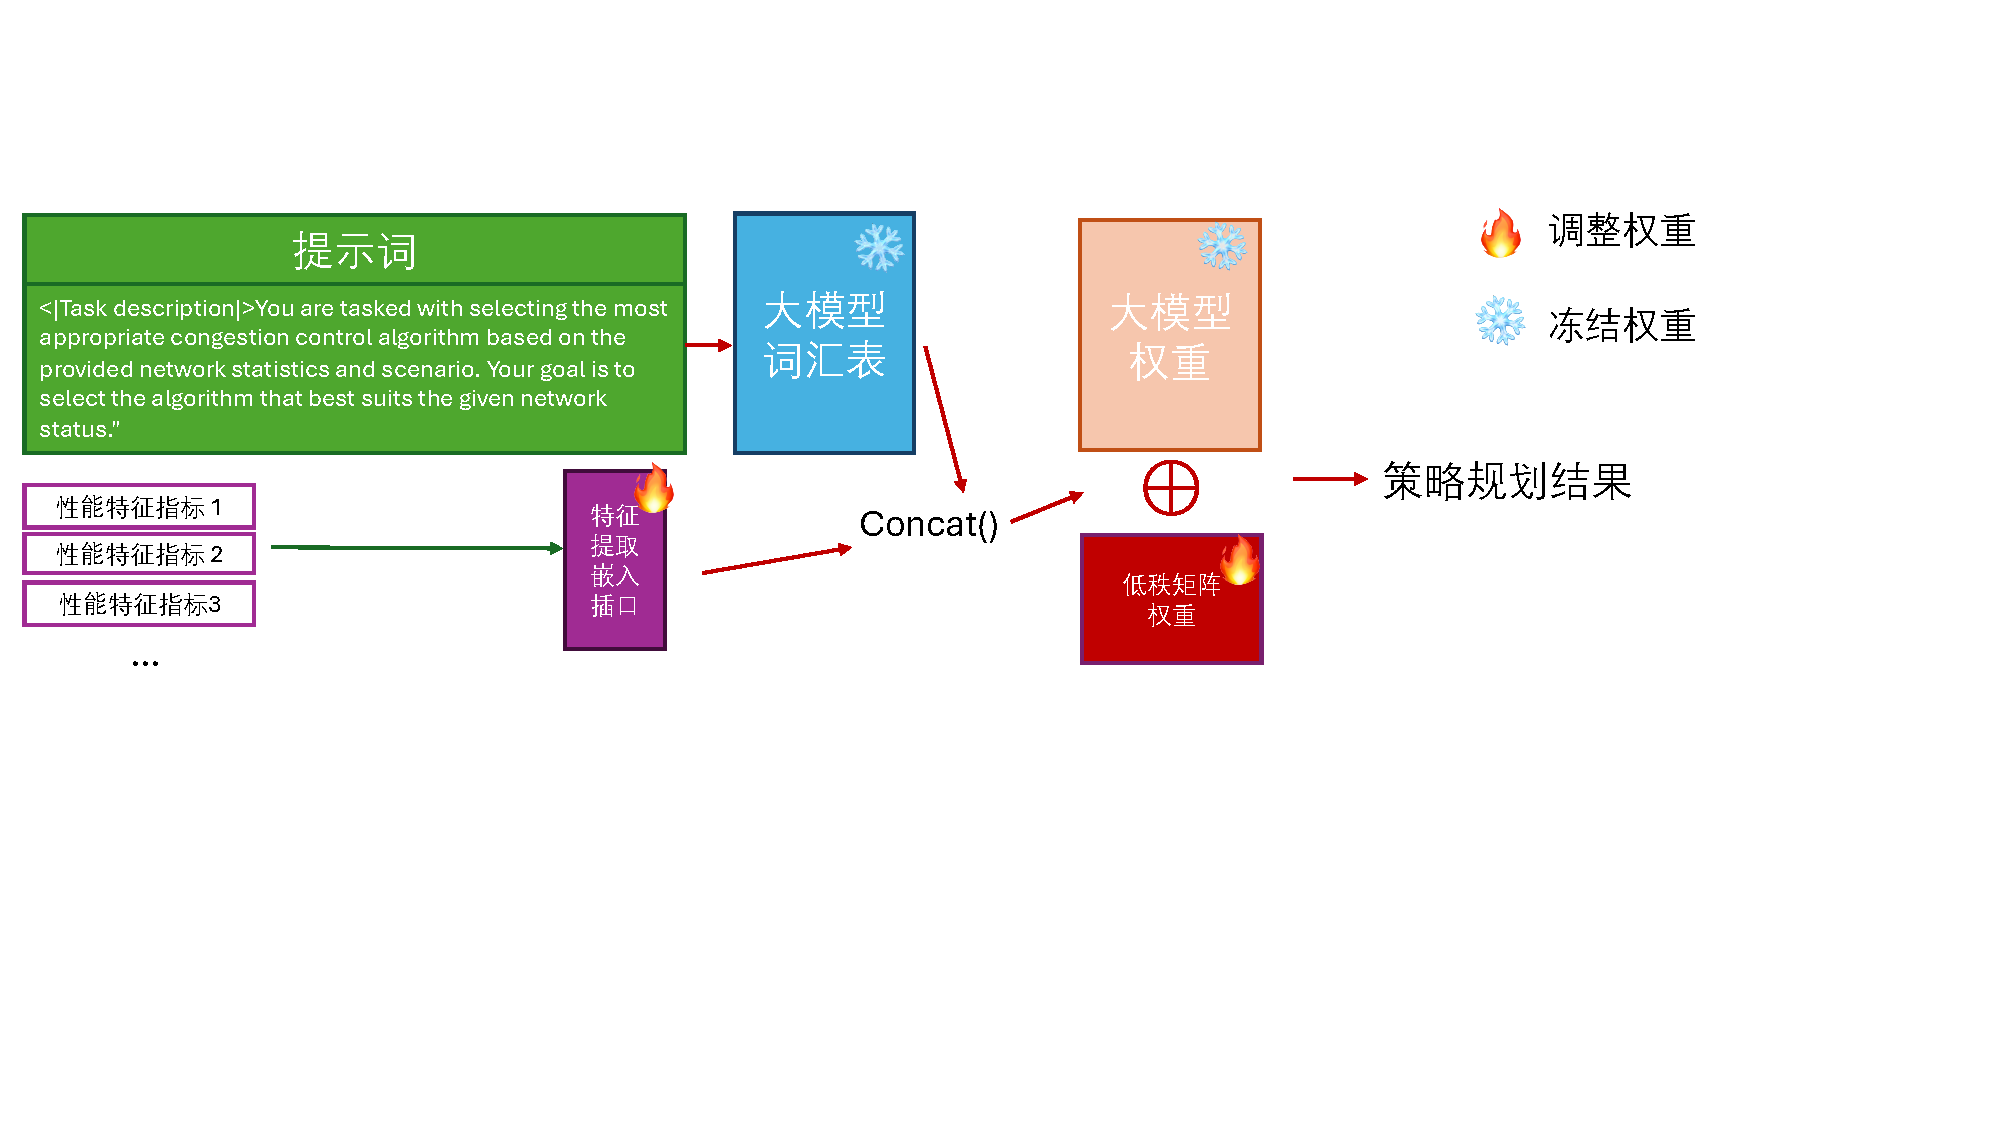
\includegraphics[width=\linewidth]{figures/chap04/model.pdf} 
\caption{LLM-NP模型的结构和权重调整情况}
\label{fig_model}
\end{figure}

\textbf{训练和学习框架:}使模型能够做出合适的策略规划决策需要在与环境交互中训练习得。解决此马尔可夫决策过程问题可以使用强化学习的方法,将任务对应的关键网络指标构成的空间视为状态空间,策略规划内容作为动作空间,并根据性能表现的结果设定奖励空间。大模型的Transformer结构使用注意力机制完成对于下一个代词(Token)的预测。在决策类任务中,Decision Transformer\cite{chen2021decision}能够提供一个适配大模型代词化输入的模型。Decision Transformer将强化学习空间中的状态(State)、动作(Action)、奖励(Reward)进行序列建模,从而给大模型符合输入要求格式、便于理解的序列,以便预测出高回报(Return)的动作。本工作使用这个方法完成前述强化问题的训练。


\textbf{数据的采集:}网络环境在运作时低容错的特性使强化学习的智能体在对应的环境中实时交互变得困难。因此使用离线的强化学习方式展开数据采集是更加合适的。离线强化学习的数据使用具体的网络任务进程给出的反馈作为数据源,并构建一个随机决策器在固定间隔内做出一个算法决策。这些决策以网络任务具体的阶段作为节点进行评估,评估方法采用任务对应的有效评估指标对一段时间内的决策效果给出可以量化的评估结果。大量这样的数据在环境中生成,然后经过一个过滤器留下评估分数最佳的前 $\alpha$\% 策略规划轨迹,作为模型的训练数据源。$\alpha $值的大小根据训练后评估实际效果、所需数据量以及工程经验综合决定,一般设置在5\%-20\%。

\textbf{训练、验证和仿真:}训练模型和验证模型使用离线数据,而仿真则在网络环境下运行和决策。训练时,进程单独运行,以损失函数值为目标优化;而仿真时,网络任务的性能指标作为评估结果直观地反馈运行结果。

具体的工作算法和流程如算法\ref{algo_proc}所示。


\begin{algorithm}
\caption{规划与网络任务控制流程}
\label{algo_proc}
\begin{algorithmic}[1]
% \STATE \textbf{输入:} 网络变化趋势嵌入接口, 预训练模型权重
% \STATE \textbf{输出:} 网络规划结果, 网络状态统计信息

\STATE \textbf{规划流程}:
\STATE 配置网络分析嵌入接口
\STATE 加载模型权重

\WHILE{接收到状态回报}
    \STATE 网络规划
    \STATE 发送网络规划结果
\ENDWHILE

\STATE \textbf{网络任务控制流程}:
\STATE 执行网络任务

\WHILE{固定粒度的时刻到达}
    \STATE 采集网络状态信息
    \STATE 发送网络状态统计信息
\ENDWHILE

\STATE \textbf{异步线程执行}:
\WHILE{收到发送结果}
    \STATE 根据规划结果开始切换算法
\ENDWHILE

\end{algorithmic}
\end{algorithm}

\subsection{模型对网络变化趋势感知}
模型对于网络变化趋势的感知和分析在强化学习的框架下将被抽象为动作、状态和奖励值。这些变量又在Decision Transformer的框架下需要抽象为符合大模型输入的序列。该工作在此过程中定义任务嵌入插口。通过任务嵌入插口,该范式支持将具体的性能指标和网络状态映射到大模型的嵌入层。无论是何种指标,每个指标经过一个多维线性层可以将低维的信息映射为大模型所需的隐藏层维度。最后,如果有多个维度的指标,将所有维度的指标连接起来,就可以形成符合大模型输入的序列。这适用于离散状态、动作和奖励空间的表示。如果空间是连续的,可以直接采用嵌入层映射到对应的维度,完成模型对网络变化趋势的感知和分析。

这样做可以实现任务规划的切换。对于不同的任务,切换对应的嵌入层就可以完成此任务的专业规划。这种方式非常灵活,就像插座的接口一样,将合适的嵌入层插入到大模型基座上,实现了任务嵌入插口。

除此外,该工作尝试将离散动作的任务作为新增的代词(Token),扩展了大模型的词汇表,这种方式有助于动作的语义理解,并为增加归因解释奠定了基础。

\subsection{案例研究:自适应码率任务下的范式应用}
为评估该范式的工作性能与效果,在本研究中寻找到一个具体的应用案例用于具像化其工作的流程和方法,即自适应码率任务。自适应码率任务的工作过程是在流式视频的传输过程中,根据实时网络的情况调整发送视频块的码率。一个完整的视频会被分为许多个块(Chunk),每个块包含了1-5秒的数据。同时,为了适配不同的终端和网络环境,每个块会以几种不同的码率展开编码,例如750Kbps, 1000Kbps, 1500Kbps。通常来说,编码的码率越高,意味着画面的清晰度、分辨率、帧率更高,进而带来更好的用户观看体验。但是网络传输性能是其中一个重要制约。如果发送了超过短时内网络承载能力数据量的块,就会导致丢包,进而造成视频的缓冲区迅速用尽,视频需要暂停重新加载,造成观看体验不佳。因此,对每个块选择合适的发送速率是观看体验的重要保证。

\subsubsection{模型建立和强化学习空间定义}
状态空间$\mathcal{S}$:自适应码率对网络变化趋势的感知需要考虑过去一段时间内的信息,该工作参考Pensieve\cite{mao2017neural},选择了过去时刻$t$的发送比特率吞吐量$x_t$、块下载时间延迟$\tau_t$、缓冲区大小变化$b_t$、和剩余的发送块的数量$c_t$和码率$l_t$信息作为特征信息。这些信息构成了多维度的状态向量,即 $\boldsymbol{s_t} = (x_t, \tau_t, b_t, c_t, l_t)$。设当前时刻为$T$,将所有特征延续采集过去5个块的时间状态作为变化趋势的分析源,即$t = T, T-1, ..., T-4$,构成矩阵$\mathcal{S}t = (\boldsymbol{s}_T, \boldsymbol{s}_{T-1}, ..., \boldsymbol{s}_{T-4})$。


动作空间$\mathcal{A}$:作为宏观的网络规划器,LLM-NP的任务主要是负责在需要的时机作出策略的调整,因此动作空间由离散的策略构成,具体策略需要网络规划流程所支持切换的策略构成。在本案例中,包括Pensieve、Genet、MPC、BBA、udr几种不同原理的策略,构成其动作空间。

奖励空间$\mathcal{R}$:在本案例中奖励值需要在训练时给出切换性能的评估。具体的评估方法采取式\eqref{eq:abr_cum_reward}所示的评估方案,考虑一段时间内的累计奖励作为决策的评估,分数越高代表性能越好。

\subsubsection{网络变化趋势感知插口的定义}
所有上述值经归一化后接入该任务对应的任务嵌入插口。对每个状态特征使用一个线性层映射到与大模型隐藏层维度一致的高维向量上;对离散的动作空间使用一个线性层作出同样的映射;而对连续的归一奖励值使用Embedding模块直接将数字进行编码映射。

所有以上的嵌入后向量在进入Decision Transformer前,还需要配置架构的上下文窗口长度$w$。该配置是为了进一步堆叠多轮的$(\mathcal{R},\mathcal{S},\mathcal{A})$以符合Decision Transformer所需要的序列输入,并设定好预期的目标回报值。在本自适应码率任务案例中,根据其工作任务的具体时长及所需的决策间隙,取窗口长度$w = 8$,即$(\mathcal{R}_t,\mathcal{S}_t,\mathcal{A}_t,\mathcal{R}_{t-1},\mathcal{S}_{t-1},\mathcal{A}_{t-1},...\mathcal{R}_{t-7},\mathcal{S}_{t-7},\mathcal{A}_{t-7})$。目标回报值取离线数据集的总奖励值25\%百分位作为模型训练时采取的目标奖励。


\subsubsection{网络与决策系统的策略选择和交互机制}
为了便于评估效果和采集训练数据,需要按照算法\ref{algo_proc}的网络规划流程调整自适应码率系统的运行环境,向规划进程提供状态信息接口,并实现事件触发策略在运行过程中无干扰切换的机制。状态信息接口可以通过在运行时添加额外的记录动作来完成。通过在进程中开辟一个专用于存储短时内程序运行状况的缓存,并在对应的数据采集点加入探针记录,可获取到对应的信息。随后缓存内容定期通过独立的通信线程与规划进程展开通信。而切换机制涉及到两个细节:(1) 如果要实现在工作时不打断的切换,需要将切换进程逐渐过渡到新的模型上。如果有权重需要加载,则在新线程中加载;(2) 如果有算法的初始量需要初始化,等待初始化完成后替换原决策策略,完成切换。在本案例中,相关的环境在pensieve的开源仿真环境上修改得来。该仿真环境使用了mahi-mahi进行端到端的网络模拟,模拟现实世界真实网络中采集的网络动态变化信息。除外,有完全仿真的相关的播放进程和发送服务器进程进行数值仿真。相关的探针和缓存空间、通信进程已在相关位置修改。

规划进程监听网络进程给出的状态信息,作出推理并发送选择的动作结果。在本案例中,模型的动作会是一个具体的算法选择,例如“genet”,“bba”。

规划进程和网络任务进程的通信方式可以视实际部署情况而定,支持网络Socket通信、共享内存通信和文件交换通信。当决策进程单独运行于独立服务器上而服务器集群间共享一个局域网时,可以依靠网络Socket进行通信,这种通信方式适合大型数据中心的部署;共享内存通信和文件交换通信则更适配在同一主机上的两个进程。

\subsubsection{模型规划能力的习得和调优}
要获得一个做出能够合理规划网络、性能表现优异的算法,需要对模型进行微调对齐,使模型适配前序系列建模的输入,并支持指定格式的输出。为了更高效、低成本地完成训练,我们采用了低秩矩阵自适应(Low Rank Adaption,LoRA)的方式,对大模型的局部权重进行微调。LoRA模型可以将高维度的矩阵通过两个低维度的满秩矩阵相乘得到,大大减小了权重的存储占用空间开销。 进行模型对齐训练时所采用的数据源从修改后的网络规划系统中获得。通过采集大量的策略切换规划序列,并根据其性能表现进行奖励值的计算,进行高奖励值的排序和筛选,留下有价值的筛选结果用于后续训练。


\section{策略规划范式和自适应码率仿真系统实现与部署}
LLM-NP范式在自适应码率任务上展开了完整的部署以评估其性能。部署部分由策略规划范式和自适应码率仿真系统两个模块构成。这些模块被部署在一台含有一块可用显卡为 NVIDIA A100-PCIE-40GB,CPU为Intel(R) Xeon(R) Gold 5318Y CPU @ 2.10GHz的服务器上.

\textbf{策略规划器的构建和训练。}策略规划器的模型权重采用开源Llama-2模型,参数量为70亿(7B),并使用Torch开源库完成模型框架、训练推理过程(包括前向传播、反向传播和梯度下降的过程);在处理预训练模型的分词(Tokenize)、令牌嵌入、增加自定义词表时使用了Huggingface平台提供的分词器和嵌入层调用接口。模型接入了自适应码率任务对应的插口,适配了自适应码率所需的网络状态信息的输入,并通过线性层映射输出头对策略规划器经过注意力机制后的所选择网络算法标签进行输出。

\textbf{自适应码率仿真系统的构建。}自适应码率仿真系统使用NetLLM\cite{wu2024netllm}和Genet\cite{xia2022genet}中提供的环境仿真器,完善仿真器的算法切换过程,增加对运行过程中更换算法的过程,以及在固定时间节点(选择时间间隔为每5个chunk)状态汇报网络状况的过程。


\textbf{策略规划器与自适应码率仿真系统的交互和推理过程。}策略规划器与自适应码率仿真系统在服务器上部署时使用文件交换的方式完成两进程之间的数据交换。同时对每个模块增加相应监听和发送线程,在不阻断模块本身功能的前提下完成信息交换。

\textbf{Decision Transformer的部署实现。}强化学习使用Decision Transformer实现,为实现该模型,按照论文\cite{chen2021decision}提供的原理将状态特征、动作和奖励分别通过线性层或嵌入层嵌入后将张量拼接。
\section{实验评估方法与实验结果}
\subsection{流程范式工作评估方法}
为了完成对新范式工作效果评估,本工作设定了完善的评估环境,以衡量规划范式的工作为相关的网络任务带来的提升,具体的网络任务为自适应码率任务。评估方法中重要的关注点包括数据集、基线对比和评估的性能指标。

\textbf{网络仿真数据集:}为了评估在具有差异化的网络环境中的运行效果,评估使用了多种状态下不同类型的真实采集网络,包括:不同的接入点和接入环境(例如公交车、地铁、汽车),以及访问不同内容提供商网络(例如Amazon,Yahoo,FaceBook)的真实访问时网络带宽记录。数据集包括以1秒或500毫秒为最细间隔粒度的对应时刻的带宽变化值,并将此网络变化文件加载在mahi-mahi中展开端到端仿真。



\textbf{预训练模型训练数据集:}预训练模型的数据集通过在网络环境上通过运行随机的算法切换并筛选性能后获得。使用的算法包括基于规则的BBA、MPC、BOLA,使用强化学习的Genet,udr\_1,udr\_2,udr\_3算法,采集了约160万个切换节点,并筛选了奖励值前6\%的数据,即约96000条训练数据。

\textbf{对比基线:}
使用的对比基线是与在传统的范式中常规算法在网络环境下的工作性能对比,以及一个简单的基于规则展开规划的算法进行性能对比而得来。
\begin{itemize}
    \item 传统范式常规算法:是指常规的网络任务运行范式中,使用的单一运行算法表现出来的性能,包括所有前述的采集数据时使用的算法。
    
    \item 基于规则展开规划的算法:使用简单的奖励值判断,如果出现突发低于前平均值的30\%,则展开随机的算法切换。
\end{itemize}

\textbf{评估的性能指标:}
在评估性能时,我们采用了自适应码率中被广泛使用的评估指标进行分数计算,它考虑了所有可能影响到内容呈现过程中用户体验的部份,包括因缓存区内缓存内容不足导致的视频重加载次数$Rebuf$,直接影响画面质量和清晰度的比特率$Bitrate$和由动态比特率切换带来的画面变动造成体验下降。整体计算方法如式\eqref{eq:abr_cum_reward2}所示,通过将各个因素加权后完成总奖励值的计算:

\begin{equation}
\begin{aligned}
    Reward = \sum_i(\alpha \cdot Rebuf_i + \beta \cdot Bitrate_i + \gamma \cdot BitrateChange_i) \cdot \frac{1}{n}
\end{aligned}
\label{eq:abr_cum_reward2}
\end{equation}

公式中的$i$代表某一个视频块(Chunk),$n$代表一次视频播放过程中的总视频块数量。公式对单个播放段内所有视频块进行汇总加权求和得到最终奖励分数。其中每一项的权重由工程经验确定,Genet\cite{xia2022genet}中线性QoE的权重,即$\alpha = -10, \beta = 1, \gamma = -1$。

\subsection{流程范式实验结果}
\textbf{LLM-NP的累计奖励值表现与其他算法对比:}本研究首先展开了在不同带宽类型下的LLM-NP的性能表现测试,并使用式\eqref{eq:abr_cum_reward2}定义的奖励值展开评估。性能表现测试的结果如图\ref{fig:multi-algo-eva}所示,对应三种类型的网络。
\begin{figure}[ht]
\centering
\begin{subfigure}[t]{0.47\linewidth}
  \centering
  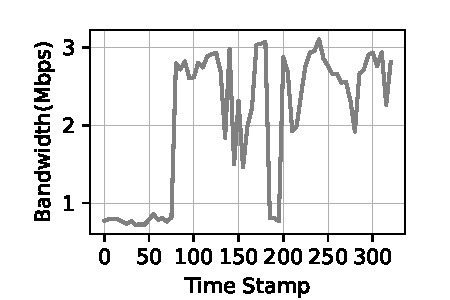
\includegraphics[width=\linewidth]{figures/chap04/evaluation_multialgo/bandwidth_68_plot.pdf}
  \caption{类型1带宽随时间变化}
  \label{type1-band-eva}
\end{subfigure}%
\begin{subfigure}[t]{0.47\linewidth}
  \centering
  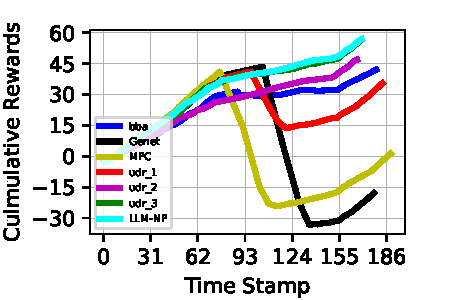
\includegraphics[width=\linewidth]{figures/chap04/evaluation_multialgo/test_68_plot.pdf}
  \caption{类型1下LLM-NP性能表现奖励值}
  \label{type1-rew-eva}
\end{subfigure}

\begin{subfigure}[t]{0.47\linewidth}
  \centering
  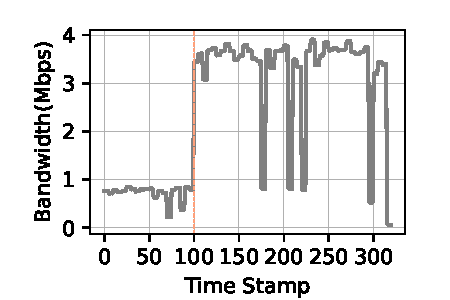
\includegraphics[width=\linewidth]{figures/chap04/evaluation_multialgo/bandwidth_27_plot.pdf}
  \caption{类型2带宽随时间变化}
  \label{type2-band-eva}
\end{subfigure}%
\begin{subfigure}[t]{0.47\linewidth}
  \centering
  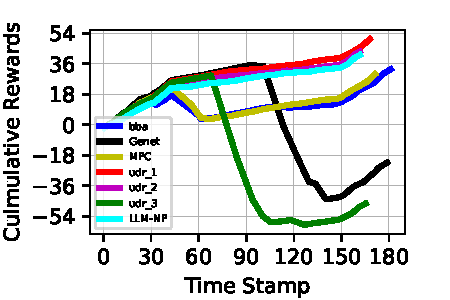
\includegraphics[width=\linewidth]{figures/chap04/evaluation_multialgo/test_27_plot.pdf}
  \caption{类型2下LLM-NP性能表现奖励值}
  \label{type2-rew-eva}
\end{subfigure}

\begin{subfigure}[t]{0.47\linewidth}
  \centering
  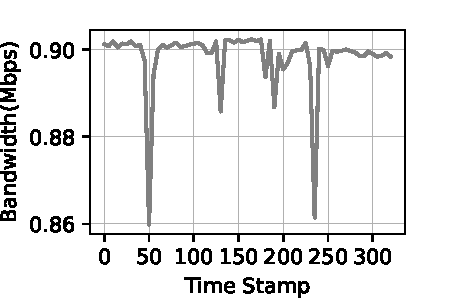
\includegraphics[width=\linewidth]{figures/chap04/evaluation_multialgo/bandwidth_88_plot.pdf}
  \caption{类型3带宽随时间变化}
  \label{type3-band-eva}
\end{subfigure}%
\begin{subfigure}[t]{0.47\linewidth}
  \centering
  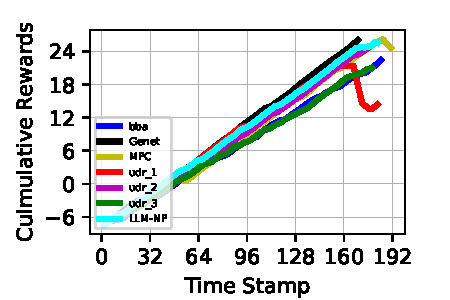
\includegraphics[width=\linewidth]{figures/chap04/evaluation_multialgo/test_88_plot.pdf}
  \caption{类型3下LLM-NP性能表现奖励值}
  \label{type3-rew-eva}
\end{subfigure}

\caption{三个类型网络环境下LLM-NP与传统算法的奖励值对比}
\label{fig:multi-algo-eva}
\end{figure}


图\ref{type1-band-eva}和图\ref{type1-rew-eva}是常见波动带宽情形下LLM-NP的效果呈现。这类带宽的特点是会有较大的抖动和方差,常见于在移动网络下,例如公交上、地铁上等信号不稳定场景。示例中的带宽波形如图\ref{type1-band-eva}所示,包含约310秒的带宽仿真,表示实时可用带宽(纵轴)随着时间消耗(横轴)而呈现出的变化趋势。带宽在90秒、120秒、150秒、190秒左右时刻出现显著波动。在此带宽下对应的策略规划范式和常规无切换策略运行的效果如图\ref{type1-rew-eva}所示,该图描述了式\eqref{eq:abr_cum_reward2}计算出的累计奖励值(纵轴)随着时间消耗(横轴)而呈现出的变化趋势。累计奖励值从0开始计算,并随着每个块(Chunk)的发送开始增减。在公式中,每个块(Chunk)发送时使用的比特率越高,对应的单次奖励值增加的越多。而奖励分数的减少则是因为遇到了缓冲区的重加载(Rebuffer)和码率变换带来的体验下降,其中缓冲区的重加载带来的体验下降更多。在图中,LLM-NP(水绿色点线表示)的奖励值曲线升高平稳,并在最终获得了最高的奖励值;与之形成对比的是MPC、Genet、udr\_1算法在90秒、120秒左右都因为网络突变而产生了较大的奖励值滑落,代表最终用户体验的下降。

图\ref{type2-band-eva} 和 \ref{type2-rew-eva}是网络状况在某一时刻后可用带宽长时变化这一类型下LLM-NP的效果呈现。这类网络的特点是在某一时刻后带宽有所增加或减少。图\ref{type2-band-eva} 中的网络带宽中在100秒出现了显著的长期可用带宽增加。相应地,传统的无法作出切换的算法会在相应带宽变化前后呈现出奖励值的下降,而LLM-NP呈现了较好的稳定性,如图\ref{type2-rew-eva}所示。

图\ref{type3-band-eva} 和 \ref{type3-rew-eva}是网络状况稳定这一类型下LLM-NP的效果呈现。这种情况下,所有的工作范式都保持了比较好的工作性能,LLM-NP呈现了与其他方法一致的最优性能,如图\ref{type3-rew-eva}所示。

\textbf{LLM-NP工作时的运行比特率和算法切换:}为了衡量LLM-NP工作时的性能表现,本研究记录并分析了其在工作时的比特率变化、随时间发送块(Chunk)时获得的单个奖励值、对网络带宽的利用率和在不同算法之间的切换情况,对应情况绘制的图例如图\ref{fig:single-algo-detail}所示。

\begin{figure}[ht]
\centering
\begin{subfigure}[t]{0.47\linewidth}
  \centering
  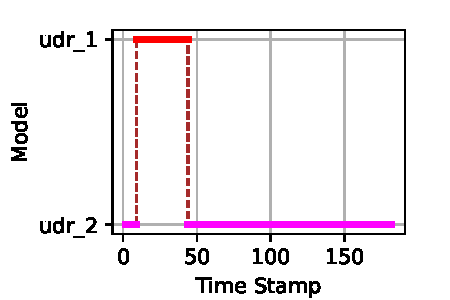
\includegraphics[width=\linewidth]{figures/chap04/evaluation_single_algo_detail/model_88_plot.pdf}
  \caption{LLM-NP工作时中的模型切换状况}
  \label{detail_model_switch}
\end{subfigure}
\begin{subfigure}[t]{0.47\linewidth}
  \centering
  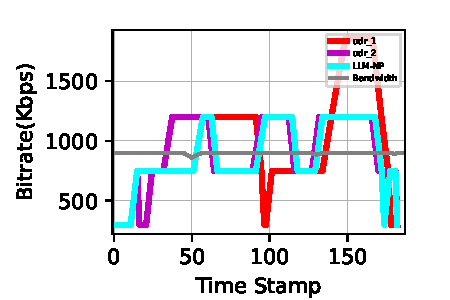
\includegraphics[width=\linewidth]{figures/chap04/evaluation_single_algo_detail/bitrate_88_plot.pdf}
  \caption{LLM-NP工作时比特率}
  \label{detail_bitrate}
\end{subfigure}%

\begin{subfigure}[t]{0.47\linewidth}
  \centering
  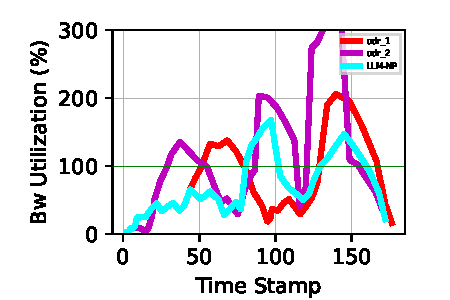
\includegraphics[width=\linewidth]{figures/chap04/evaluation_single_algo_detail/bandwidth_utilization_88_plot.pdf}
  \caption{LLM-NP工作时的带宽利用率}
  \label{detail_bandwid_util}
\end{subfigure}%
\begin{subfigure}[t]{0.47\linewidth}
  \centering
  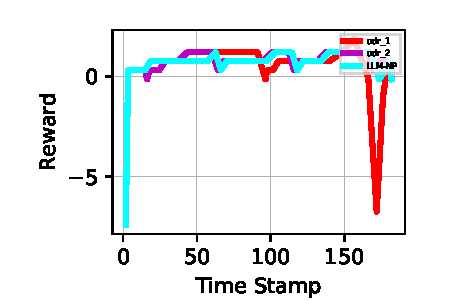
\includegraphics[width=\linewidth]{figures/chap04/evaluation_single_algo_detail/reward_88_plot.pdf}
  \caption{LLM-NP工作获得单次奖励值}
  \label{detail_reward}
\end{subfigure}

\caption{LLM-NP工作时的性能表现细节}
\label{fig:single-algo-detail}
\end{figure}


图\ref{detail_model_switch}表明了LLM-NP在本示例工作时的涉及使用的算法,包括“udr\_1”和“udr\_2”。模型在最初的10秒左右的时间中使用了“udr\_2”算法,随后切换到“udr\_1”,并在接近50秒时又切换回“udr\_2”算法并保持不变。

图\ref{detail_bitrate}代表LLM-NP工作时的发送比特率随着时间推移而选择的块(Chunk)变化值。图中灰色的线代表使用的环境模拟可用带宽,其可用带宽在900Kbps左右保持平稳;草绿色线代表LLM-NP在该任务下的比特率控制。在本次的算法规划中,算法所涉及的两个算法“udr\_1”和“udr\_2”也在图中分别以红色和紫色表示。通过该图,我们可以直观地看到LLM-NP的比特率控制相比使用单一的算法有更优的性能:“udr\_2”的算法在前40秒内的比特率较低,没有完全利用到大部份的带宽,而LLM-NP做出的切换能够有效增加带宽利用率,提升使用性能;而“udr\_1”在100秒后的比特率控制波动较大,存在较大的比特率切换,且较多超过了可用带宽,可能会导致重缓冲(Rebuffer)的产生,和较多比特率切换罚项,造成最终QoE奖励值下降。在本例中,LLM-NP相比任一单一的算法在带宽利用、比特率切换和重加载避免方面表现出了更佳的性能。

图\ref{detail_bandwid_util}代表LLM-NP工作时的带宽利用率。类似的,涉及到切换的算法也相应在图中绘制用于对比和衡量。LLM-NP相比“udr\_1”和“udr\_2”有更稳定的,接近高带宽利用率的性能。图\ref{detail_reward}代表LLM-NP工作时发送每个块(Chunk)时获得的单次奖励值。

\subsection{局限性讨论}
本章节所设计的LLM-NP范式的工作范围限定于具备庞大策略库,且对应系统能够实现运行时切换的网络任务。目前研究能够在自适应码率任务的仿真系统上实现了切换,产生初步的优化效果和相应的性能提升。然而,其效果的进一步提升与验证需要借助更大的数据量和更真实的、大规模的正式系统平台完成验证,包括在更多差异化的网络任务(例如拥塞控制、梯度压缩、实时通信发送率控制)、更全面的算法运行数据采集(多种算法的长时运行数据)、更大的预训练模型(使用更高参数量的模型)上展开验证,以及确定对应的任务在真实系统部署中切换所存在的难点。
\section{本章小结}
本章节提出了LLM-NP,一种用于网络控制的策略规划新范式。这种范式改变了过往在网络传输控制中固定一成不变的策略选择,并利用了大模型的感知和规划能力,为网络传输控制类的任务提供了可动态切换的解决方案。该工作对大模型展开了在网络任务上的具体数据上的微调对齐,并实现了网络规划范式与自适应码率任务的完整交互系统,获得了在变动网络带宽环境下,超越传统单一运行算法的可靠的性能提升案例。
